\subsection{Related Standards}
\subsubsection{C++14} 
C++ was programmed according to the C++14 standard provided by Texas Instruments' ARM compiler. This standard is formally known as \href{https://www.iso.org/standard/64029.html}{ISO/IEC 14882:2014}. C++ is a superset of C, and builds upon it by introducing object-oriented programming concepts while maintaining the functional language aspect of C.
\subsubsection{802.11} 
The microcontroller (MCU) supported transmission through the Institute of Electrical and Electronics Engineers (IEEE) 802.11b/g/n standard of wireless communication. This standard used the S band of radio frequencies and operated at 2.4 GHz. There were 14 accessible channels, each spanning a bandwidth of 22 MHz (pictured in \autoref{wifi_channels}).
\begin{figure}[H]
    \caption{802.11b/g/n channels \cite{Flickenger}}
    \label{wifi_channels}
    \centering
    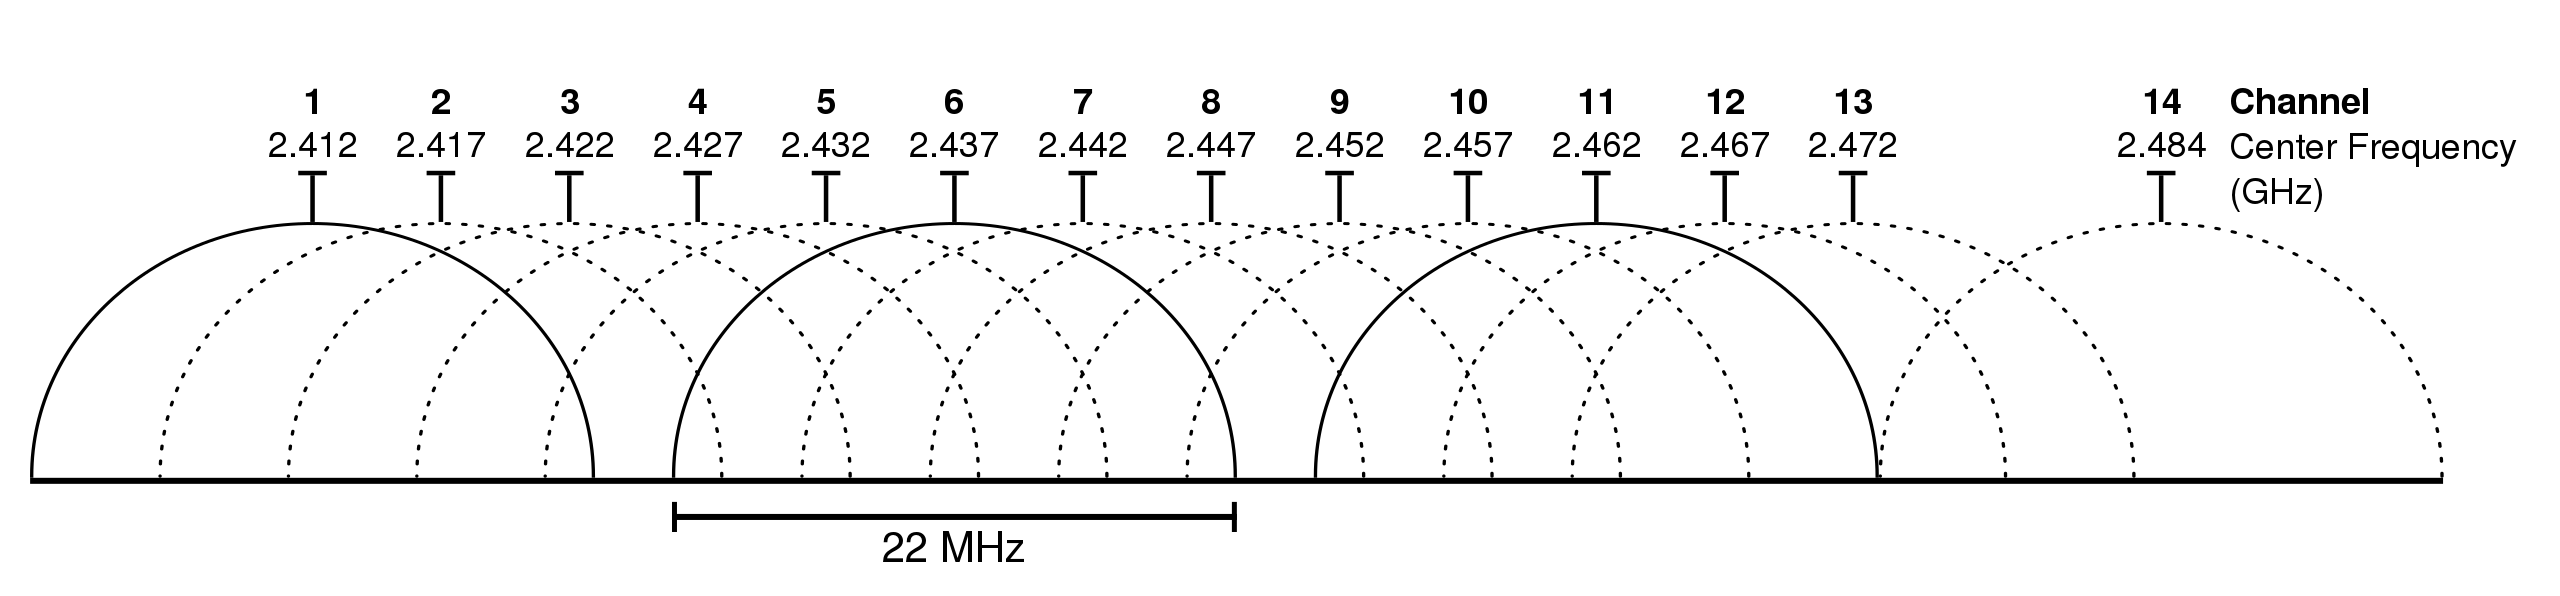
\includegraphics[width=\textwidth]{images/wifi_channels.png}
\end{figure}
These channels specifically resided in an industrial, scientific, and medical (ISM) band. This standard also provided datagram frames for the transport layer.
\subsubsection{TCP} \label{tcp_standard} 
Transmission Control Protocol (TCP) was used to satisfy the transport layer requirements of the product, and was used to transmit symbols (i.e., from any commands, data, settings, telemetry, etc.) between Amazon Web Services (AWS) and the microcontroller (MCU). TCP was chosen over other protocols, such as User Datagram Protocol (UDP), mainly due to its reliability. The extent of TCP's reliability included features such as checksums, duplicate data detection, retrying of transmissions, sequencing, and timers. Such reliability was favored over higher bandwidth or lower latency, as neither of the latter were required for the kilobytes of information being relayed between AWS and the MCU. A standard TCP frame was shown in \autoref{tcp_frame}.
\begin{figure}[H]
    \caption{TCP frame \cite{Kristoff}}
    \label{tcp_frame}
    \centering
    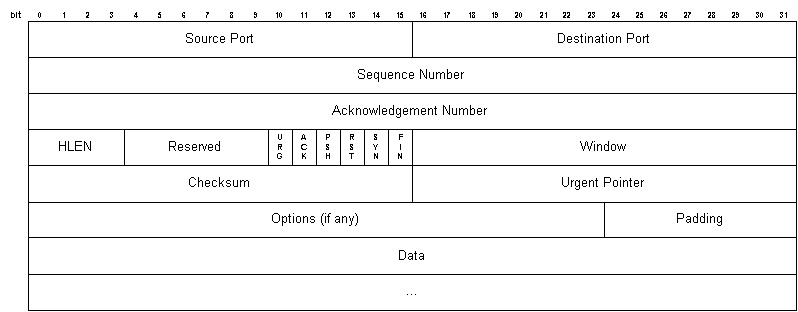
\includegraphics[width=\textwidth]{images/tcp_frame.jpg}
\end{figure}

\subsubsection{IPv4} 
IPv4 was the fourth version of the Internet Protocol, a network layer protocol in use to relay data between devices and across networks. The data relayed, datagrams, were sent between sources and hosts that were identified by 32-bit addresses. This protocol strictly functioned to transport the datagram from one device to another, with no end-to-end reliability, flow control, sequencing, or other measures found in other protocols such as TCP. IPv4 provided two distinct features: fragmentation of whole datagrams, and addressing of devices. A standard IPv4 frame was shown in \autoref{ipv4_frame}.
\begin{figure}[H]
    \caption{IPv4 frame \cite{Postel1981}}
    \label{ipv4_frame}
    \centering
    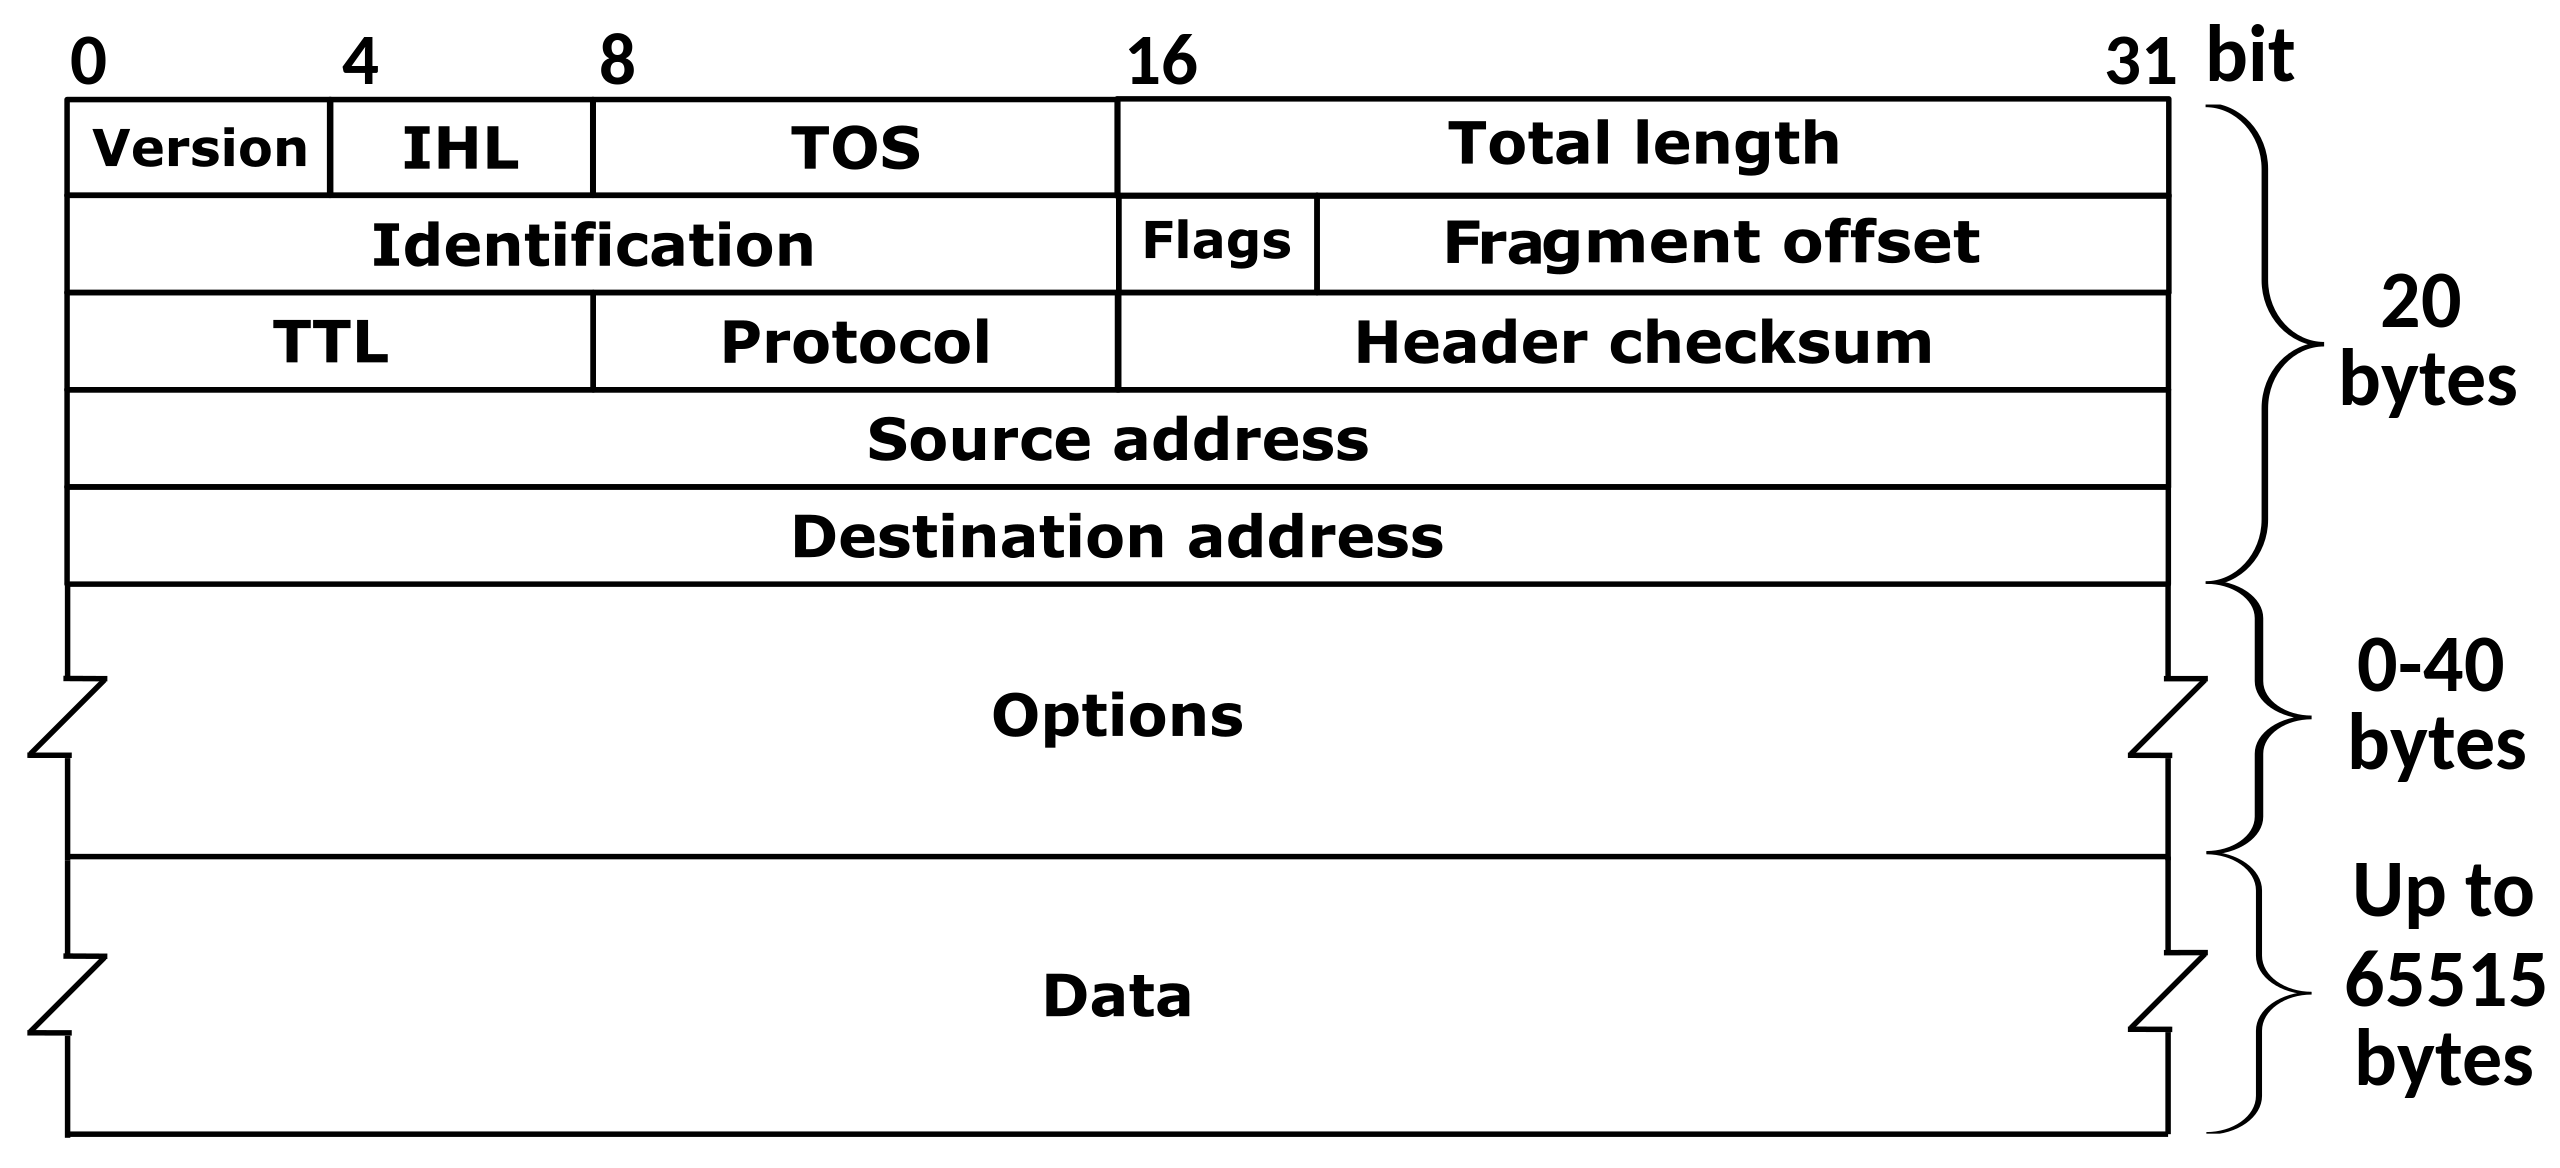
\includegraphics[width=\textwidth]{images/ipv4_frame.png}
\end{figure}